% Dokumentacja projektu — Wizja komputerowa (AGH)
% Kompilacja:  pdflatex dokumentacja.tex   (dwukrotnie, dla spisu i odnośników)
% UWAGA: limit 5 stron (z obrazami, tabelami i bibliografią włącznie).
%        Przekroczenie limitu = 0 pkt. Marginesy i odstępy są celowo zwarte.
\documentclass[10pt,a4paper]{article}

\usepackage[T1]{fontenc}
\usepackage[utf8]{inputenc}
\usepackage[polish]{babel}
\usepackage[margin=2cm]{geometry}
\usepackage{graphicx}
\usepackage{booktabs}
\usepackage{microtype}
\usepackage{siunitx}
\usepackage{caption}
\usepackage{subcaption}
\usepackage[hidelinks]{hyperref}

\captionsetup{font=small,labelfont=bf}
\setlength{\parskip}{2pt}
\setlength{\parindent}{0pt}

% Ścieżka do rysunków eksportowanych z notatnika (viz.* zwraca obiekt Figure,
% który można zapisać przez fig.savefig("docs/figures/...")).
\graphicspath{{figures/}}

\title{\vspace{-1.5em}Klasyfikacja obrazów metodami klasycznej wizji komputerowej}

\author{
    \begin{tabular}{c}
        \small Maciej Kmąk \quad \small Hubert Miklas \quad \small Mateusz Wójcik \\[0.5em]
        \small Akademia Górniczo-Hutnicza \\
        \small Systemy Wizyjne
    \end{tabular}
}

\date{}

\begin{document}
\maketitle
\vspace{-2.5em}

% ============================================================ %
\section{Wprowadzenie i zbiór danych}
% ============================================================ %
Celem projektu jest klasyfikacja obrazów wyłącznie metodami klasycznej wizji
komputerowej i uczenia maszynowego. Działanie projektu obejmuje:
wczytanie danych, preprocessing analizowanych obrazów, ekstrakcję cech, klasyfikację oraz dobór
parametrów na zbiorze treningowo-walidacyjnym i ocenę na osobnym zbiorze
testowym. Pracujemy na dwóch zbiorach zawartych w poleceniu. Pierwszy zawiera próbkę 164 obrazów treningowych jabłek i 130 obrazów treningowych zawierających zdjęcia pomidorów. Zbiór testowy zawiera odpowiednio 54 zdjęcia jabłek i 43 zdjęcia pomidorów.

\begin{figure}[htp]
    \centering
    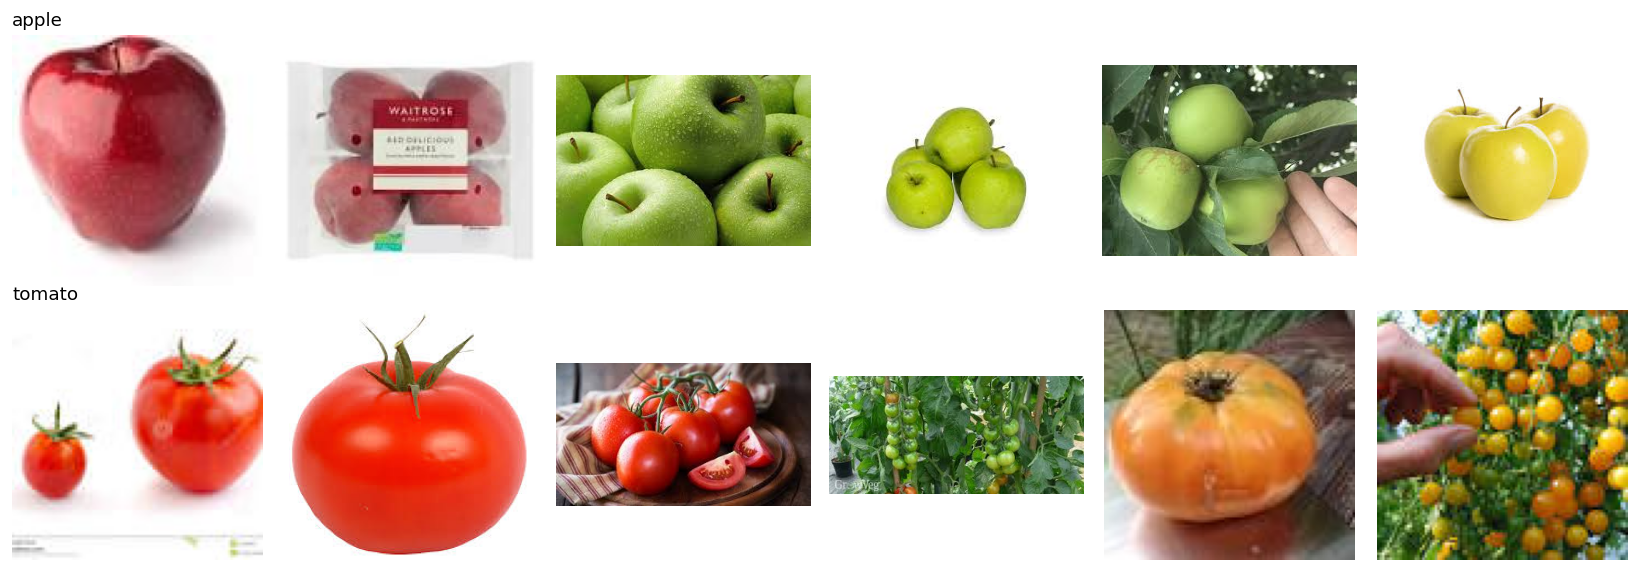
\includegraphics[width=0.7\linewidth]{apple_tomato.png}
    \caption{Przykład danych treningowych do klasyfikacji pomidorów i jabłek}
    \label{fig:wireshark}
\end{figure}

% ============================================================ %
\section{Preprocessing}
% ============================================================ %

Wszystkie obrazy przetwarzane są przez łańcuch kroków zaimplementowany
w module \texttt{preprocessing} (funkcja \texttt{preprocess}). Kolejność operacji jest
konfigurowana parametrem \texttt{steps}; Poniższy opis skupia się na wiariancie domyślnym stosowanych w tym projekcie.

\begin{itemize}\itemsep1pt

\item \textbf{Usunięcie artefaktów}

Pierwszym krokiem jest filtracja medianowa wybrana ze względu na skuteczne usuwanie szumu typu
\emph{sól i pieprz} oraz bloki kompresji JPEG. Filtr medianowy zachowuje krawędzie
obiektu lepiej niż rozmycie Gaussa, co jest kluczowe dla późniejszej segmentacji.

\item \textbf{Korekcja balansu bieli}

Zdjęcia roślin i owoców często charakteryzują się dominującą barwą, co może skutkować zaburzeniem odcieni kolorystycznych. W celu redukcji zjawiska stosowana jest metoda \emph{gray-world}, polegająca na skalowaniu każdego kanału RGB w taki sposób, aby jego średni piksel odpowiadał średniej globalnej jasności obrazu. Wyrównanie redukuje systematyczny odcień, dzięki czemu cechy koloru w tym wartości odcienia są porównywalne między obrazami.

\item \textbf{Poprawa kontrastu}

Kontrast wzmacniany jest algorytmem CLAHE (\emph{Contrast Limited Adaptive
Histogram Equalization}) z parametrami \texttt{clip\_limit}\,=\,2{,}0 i
siatką $8{\times}8$. Kluczowe jest, że w przypadku kolorowych obrazów dokonywana jest konwersja do przestrzeni LAB, a wyrównanie histogramu przeprowadzane jest wyłącznie na kanale jasności $L$, a nie na kanałach RGB oddzielnie. Dzięki temu nasycenie i barwa pozostają niezmienione, a wzmocnieniu ulega jedynie kontrast lokalny. Wybór algorytmu CLAHE jest motywowany działaniem lokalnym algorytmu, pozwalającym uzyskiwać zadowalające rezultaty zarówno na jasnych, jak i ciemnych partiach obrazu oraz odpornością na tworzenie szumów obrazu.

\item \textbf{Segmentacja obiektu od tła}

Segmentacja realizowana jest progowaniem globalnym metodą Otsu. Algorytm
automatycznie wyznacza próg podziału na podstawie histogramu jasności obrazu,
szukając takiej wartości, która najlepiej rozdziela piksele tła od pikseli
obiektu. Działa to dobrze dla zdjęć liści i owoców, gdzie obiekt i tło różnią
się wyraźnie jasnością (obiekt jest zazwyczaj ciemniejszy lub bardziej
nasycony niż jednolite tło fotografii). Jeśli większość pikseli należy do tła
(powoduje to jasną maskę), wynik jest automatycznie inwertowany, tak aby obiekt zawsze
odpowiadał wartości 255. Uzyskana maska binarna jest następnie czyszczona, poprzez użycie
otwarcia eliptycznego jądrem $5{\times}5$, co usuwa małe fałszywe plamy, a domknięcie
tym samym jądrem uszczelnia dziury wewnątrz obiektu. Na koniec zachowywana jest
wyłącznie największa składowa spójna, co eliminuje oderwane fragmenty tła
pozostałe po progowaniu.

\begin{figure}[htp]
    \centering
    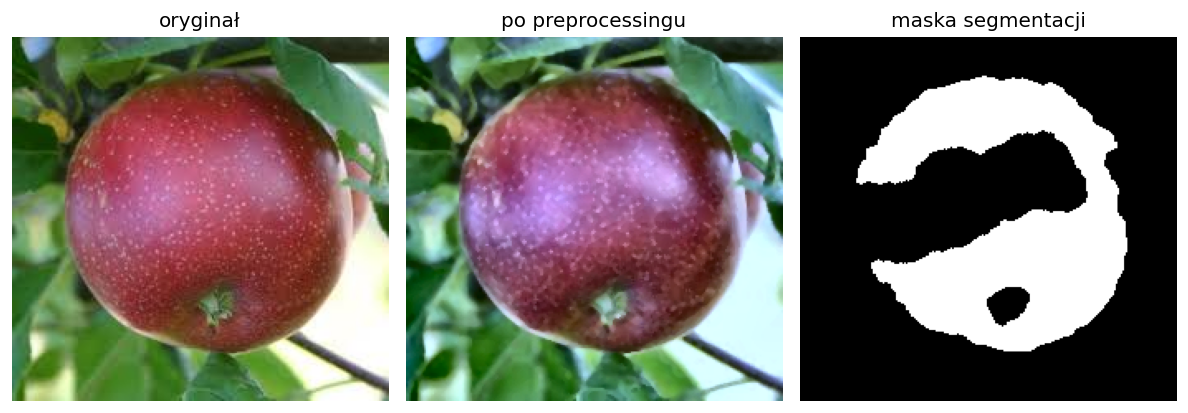
\includegraphics[width=0.7\linewidth]{preprocess.png}
    \caption{Przykład łańcucha preprocessingu: oryginał (lewo),
           obraz po korekcji kontrastu i balansu bieli (środek),
           maska segmentacji (prawo).}
    \label{fig:wireshark}
\end{figure}

\end{itemize}


% ============================================================ %
\section{Ekstrakcja cech}
% ============================================================ %
\subsection*{Ekstrakcja cech}

Każdy obraz reprezentowany jest wektorem 85 cech, łączącym trzy kategorie identyfikujące jego cechy: teksturę, kolor i kształt.

\textbf{Tekstura (GLCM, 56 cech).} Macierz współwystąpień poziomów szarości
budowana jest po uprzedniej kwantyzacji obrazu do 32 poziomów, co zapewnia
gęste wypełnienie macierzy przy ograniczonym szumie statystycznym. Obliczenia
prowadzone są dla dwóch odległości między pikselami ($d \in \{1, 3\}$) i czterech
kątów ($0°, 45°, 90°, 135°$), co pozwala uchwycić zarówno drobną, jak i grubszą
teksturę niezależnie od kierunku. Z każdej płaszczyzny wyznaczane są deskryptory
Haralicka (kontrast, niepodobieństwo, jednorodność, energia, korelacja, ASM)
oraz entropia liczona ręcznie. Cechy tekstury są szczególnie istotne przy
rozróżnianiu chorych i zdrowych liści, gdzie zmiany chorobowe tworzą
charakterystyczne, nieregularne wzory powierzchni.
\\

\textbf{Kolor (18 cech).} Dla każdego z sześciu kanałów (RGB i HSV) wyznaczane
są trzy statystyki: średnia, odchylenie standardowe i skośność rozkładu.
Obliczenia prowadzone są wyłącznie na pikselach należących do obszaru obiektu
wskazanego przez maskę segmentacji, dzięki czemu czarne tło nie zaburza
wyników. Przestrzeń HSV uzupełnia RGB, ponieważ odcień $H$ i nasycenie $S$
są bardziej odporne na zmienność oświetlenia niż surowe wartości kanałów
czerwonego, zielonego i niebieskiego.
\\

\textbf{Kształt (11 cech).} Z największego konturu wyznaczonego na masce binarnej obliczane są: pole powierzchni, obwód, średnica zastępcza (średnica koła o takim samym polu), wymiary prostokąta ograniczającego, współczynnik wypełnienia (extent), stopień upakowania (okrągłość) oraz wydłużenie (asymetria) dopasowanej elipsy. Uzupełniają je statystyki promieni od środka ciężkości (geometrycznego) do punktów konturu (maksymalny, minimalny, średni). Stopień upakowania i wydłużenie elipsy są niezależne od skali obrazu, co zabezpiecza przed wpływem różnych rozdzielczości wejściowych
% TODO: które rodziny ostatecznie użyto (use=...) i dlaczego (np. rozkłady cech).
% TODO: wstawić viz.plot_feature_distributions dla 3-4 najbardziej różnicujących cech.

\newpage
% ============================================================ %
\section{Klasyfikacja i dobór parametrów}
% ============================================================ %

Do klasyfikacji owoców (jabłka vs.\ pomidory) zastosowano pięć klasycznych
algorytmów uczenia maszynowego dostępnych w bibliotece \texttt{scikit-learn}:
maszynę wektorów nośnych (SVM), drzewo decyzyjne (\textit{Decision Tree}),
las losowy (\textit{Random Forest}), klasyfikator $k$ najbliższych sąsiadów
(kNN) oraz regresję logistyczną.
Każdy klasyfikator osadzono wewnątrz potoku (\texttt{Pipeline}) poprzedzonego
standaryzacją cech (\texttt{StandardScaler}).
Skalowanie jest niezbędne dla metod opartych na odległości - SVM i kNN -
ponieważ wyekstrahowane rodziny cech operują na bardzo różnych skalach wartości:
cechy tekstury GLCM mieszczą się w przedziale $[0, 1]$, podczas gdy deskryptory
kształtu takie jak pole powierzchni (\textit{area}) osiągają wartości rzędu
tysięcy pikseli.
Umieszczenie skalera \emph{wewnątrz} potoku gwarantuje, że parametry
normalizacji są wyznaczane wyłącznie na foldzie treningowym, co eliminuje
wyciek informacji z~danych walidacyjnych.
\\

Dobór hiperparametrów przeprowadzono metodą przeszukiwania siatki
(\texttt{GridSearchCV}
(\texttt{StratifiedKFold}).
Kryterium optymalizacji stanowiła miara $F_1$ uśredniona makro, która
równomiernie penalizuje błędy na każdej klasie niezależnie od jej liczebności.
Dla SVM przeszukiwano kombinacje parametru regularyzacji
$C \in \{0.1, 1, 10, 100\}$, szerokości jądra RBF
$\gamma \in \{\texttt{scale}, 0.01, 0.001\}$ oraz typu jądra
(\texttt{rbf}, \texttt{linear}).
Dla drzewa decyzyjnego testowano maksymalną głębokość
$d \in \{5, 10, 20, \infty\}$, minimalną liczbę próbek w liściu
$n_\text{leaf} \in \{1, 2, 5\}$ oraz kryterium podziału (Gini / entropia).
Las losowy strojono w zakresie liczby drzew $\{100, 200, 400\}$, maksymalnej
głębokości oraz liczby cech rozważanych w węźle (\texttt{sqrt}, \texttt{log2}).
Zbiór danych był dostarczony z~gotowym podziałem na podzbiór treningowy i
testowy (\texttt{presplit = True}), dlatego walidacja krzyżowa odbywała się
wyłącznie w obrębie zbioru treningowego, a wyniki końcowe wyznaczano na
wydzielonym zbiorze testowym.

Zmieniłem temat na jabłka vs. pomidory i dodałem wzmiankę o gotowym podziale train/test (presplit = True), który jest charakterystyczny właśnie dla tego datasetu.

% ============================================================ %
\section{Wyniki i krytyczna analiza}
% ============================================================ %
Końcową ocenę przeprowadzono \emph{raz}, na wydzielonym zbiorze testowym.
Tabela~\ref{tab:wyniki} zestawia metryki; raportujemy średnie makro
(traktują klasy równo) oraz ważone.

\begin{table}[h]
  \centering\small
  \caption{Metryki na zbiorze testowym. % TODO: uzupełnić liczbami z metrics.compare_models
  }
  \label{tab:wyniki}
  \begin{tabular}{lcccc}
    \toprule
    Model & Accuracy & Precision\textsubscript{macro} & Recall\textsubscript{macro} & F1\textsubscript{macro} \\
    \midrule
    SVM              & -- & -- & -- & -- \\
    Drzewo decyzyjne & -- & -- & -- & -- \\
    Las losowy       & -- & -- & -- & -- \\
    \bottomrule
  \end{tabular}
\end{table}

\begin{figure}[h]
  \centering
  % TODO: viz.plot_confusion_matrix(...) -> fig.savefig("figures/confusion.png")
  \fbox{\parbox[c][2.6cm][c]{0.5\linewidth}{\centering\small
    [Rys.~--- macierz pomyłek najlepszego modelu]}}
  \caption{Macierz pomyłek najlepszego klasyfikatora na zbiorze testowym.}
  \label{fig:cm}
\end{figure}

\textbf{Analiza.} % TODO: napisać autorskie wnioski (najważniejsza część oceny):
% - która rodzina cech daje największy wkład (feature importance / rozkłady)?
% - które klasy są mylone i dlaczego (off-diagonal macierzy pomyłek)?
% - rozbieżność accuracy vs F1_macro przy niezbalansowanych klasach?
% - wpływ preprocessingu/segmentacji na wynik (ablacja)?
[do uzupełnienia po eksperymentach]

% ============================================================ %
\section{Wnioski}
% ============================================================ %
% TODO: 3-5 zdań podsumowania: najlepsza konfiguracja, ograniczenia, co dalej.
[do uzupełnienia]

% ============================================================ %
\begin{thebibliography}{9}
\small
\bibitem{haralick} R.~M. Haralick, K.~Shanmugam, I.~Dinstein,
  \emph{Textural Features for Image Classification}, IEEE TSMC, 1973.
\bibitem{skimage} S.~van der Walt i in.,
  \emph{scikit-image: image processing in Python}, PeerJ, 2014.
\bibitem{sklearn} F.~Pedregosa i in.,
  \emph{Scikit-learn: Machine Learning in Python}, JMLR, 2011.
\bibitem{opencv} G.~Bradski, \emph{The OpenCV Library}, Dr.~Dobb's Journal, 2000.
% TODO: dodać źródło zbioru danych (np. PlantVillage) oraz pozostałe odnośniki.
\end{thebibliography}

\end{document}